\section{Group -- Plant-Condenser Loops}\label{group-plant-condenser-loops}

\subsection{PlantLoop}\label{plantloop}

The main elements of the PlantLoop syntax are described in further detail below. A map of how the input for this portion of the HVAC input fits together is provided in the following diagram.

\begin{figure}[hbtp] % fig 73
\centering
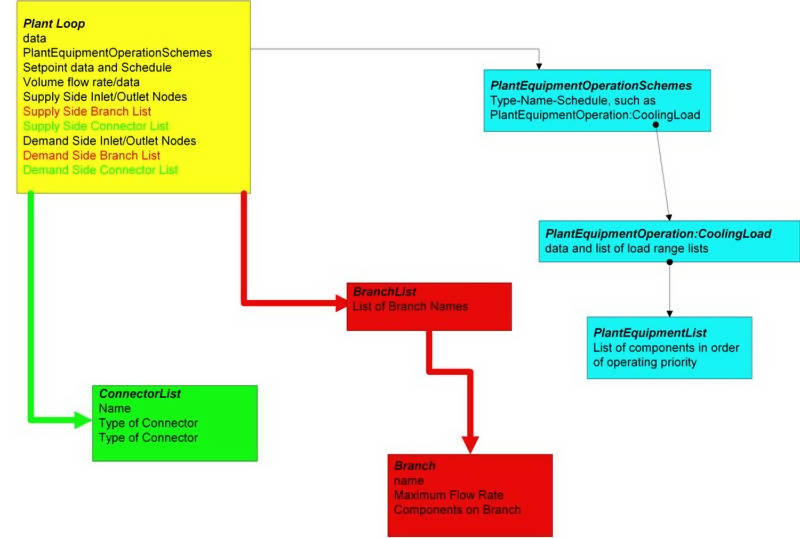
\includegraphics[width=0.9\textwidth, height=0.9\textheight, keepaspectratio=true]{media/image135.png}
\caption{Plant Loop Input Syntax Map \protect \label{fig:plant-loop-input-syntax-map}}
\end{figure}

\subsubsection{Inputs}\label{inputs-035}

\paragraph{Field: Name}\label{field-name-034}

This alpha field is used as an identifying field for the plant loop.

\paragraph{Field: Fluid Type}\label{field-fluid-type-001}

This alpha field must be a keyword selected from the list of available fluids for an EnergyPlus plant loop. Either \textbf{Water}, \textbf{Steam} or \textbf{UserDefinedFluidType} may be used. If the UserDefinedFluidType keyword is used, the following input field i.e.~User Defined Fluid Type must have a value (namely the name of a \hyperref[fluidpropertiesglycolconcentration]{FluidProperties:GlycolConcentration} object).

\paragraph{Field: User Defined Fluid Type}\label{field-user-defined-fluid-type-000}

This alpha field must be specified when the previous field is set to \textbf{UserDefinedFluidType} otherwise it could be left blank. \textbf{Water}, \textbf{EthyleneGlycol}, \textbf{PropyleneGlycol} and \textbf{Steam} are all ``built-in'' fluids for EnergyPlus (that is, all of the appropriate properties are contained within the program). If the fluid specified here is a mixture of water and ethylene or propylene glycol, then only \hyperref[fluidpropertiesglycolconcentration]{FluidProperties:GlycolConcentration} objects need to be specified and the name of the appropriate one is used here. For another water/glycol mixture, a complete set of fluid property data (\hyperref[fluidpropertiesname]{FluidProperties:Name} and FluidProperties:Temperature objects plus multiple \hyperref[fluidpropertiesconcentration]{FluidProperties:Concentration} objects for specific heat, density, etc.) must be specified (Ref dataset: GlycolPropertiesRefData.idf).

\paragraph{Field: Plant Equipment Operation Scheme Name}\label{field-plant-equipment-operation-scheme-name}

This alpha field is used as an identifying field for the plant operation scheme. This field ties to the \hyperref[plantequipmentoperationschemes]{PlantEquipmentOperationSchemes} input structure, which must also be defined.

\paragraph{Field: Loop Temperature Setpoint Node Name}\label{field-loop-temperature-setpoint-node-name}

This alpha field is used to identify the node which the Loop Manager will access the temperature setpoint that it will try to maintain. This is typically the Plant Loop Supply Side Outlet Node so that it will not interfere with component temperature setpoints. An associated temperature setpoint manager will need to be defined.

\paragraph{Field: Maximum Loop Temperature}\label{field-maximum-loop-temperature}

This numeric field contains the maximum allowable temperature in Celsius for this loop.

\paragraph{Field: Minimum Loop Temperature}\label{field-minimum-loop-temperature}

This numeric field contains the minimum allowable temperature in Celsius for this loop.

\paragraph{Field: Maximum Loop Flow Rate}\label{field-maximum-loop-flow-rate}

This numeric field contains the maximum loop flow rate in cubic meters per second. This parameter is also used when the user chooses to autocalculate the loop volume. See Volume of the Plant Loop below and the Engineering Manual for more details. This field is autosizable.

\paragraph{Field: Minimum Loop Flow Rate}\label{field-minimum-loop-flow-rate}

This numeric field contains the minimum loop flow rate in cubic meters per second.

\paragraph{Field: Plant Loop Volume}\label{field-plant-loop-volume}

Volume of the plant loop in m\(^{3}\). This numeric field contains the loop volume for the entire loop, i.e.~both the demand side and the supply side. This is used for the loop capacitance calculation. Loop volume (m\(^{3}\)) could be calculated from pipe size data but this is not usually known. If zero volume is specified the loop has no fluid heat capacity. If a very large capacitance is specified unrealistic time delay may result and there may be poor response to changes in loop setpoint temperature. The \textbf{autocalculate} option sets the loop volume to the product of the Maximum Loop Flow Rate and the user input for Loop Circulation Time which defaults to 2 minutes (see below). This calculation is described in the Engineering Reference manual.

\paragraph{Field: Plant Side Inlet Node Name}\label{field-plant-side-inlet-node-name}

This required alpha field contains the identifying name given to the Plant Side Inlet Node.~ This node is the inlet to the supply side of the loop.

\paragraph{Field: Plant Side Outlet Node Name}\label{field-plant-side-outlet-node-name}

This required alpha field contains the identifying name given to the Plant Side Outlet Node. This node is the outlet of the supply side of the loop.

\paragraph{Field: Plant Side Branch List Name}\label{field-plant-side-branch-list-name}

This required alpha field contains the identifying name given to the Plant Side Branch List. The list referenced here should list all the branches on the supply side of the loop.

\paragraph{Field: Plant Side Connector List Name}\label{field-plant-side-connector-list-name}

This alpha field contains the identifying name given to the Plant Side Connector List. The list referenced here should list the splitter and mixer on the supply side of the loop.

\paragraph{Field: Demand Side Inlet Node Name}\label{field-demand-side-inlet-node-name}

This required alpha field contains the identifying name given to the Demand Side Inlet Node. This node is the inlet to the demand side of the loop.

\paragraph{Field: Demand Side Outlet Node Name}\label{field-demand-side-outlet-node-name-000}

This required alpha field contains the identifying name given to the Demand Side Outlet Node. This node is the outlet of the demand side of the loop.

\paragraph{Field: Demand Side Branch List Name}\label{field-demand-side-branch-list-name}

This required alpha field contains the identifying name given to the Demand Side Branch List. The list referenced here should list all the branches on the demand side of the loop.

\paragraph{Field: Demand Side Connector List Name}\label{field-demand-side-connector-list-name}

This alpha field contains the identifying name given to the Demand Side Connector List. The list referenced here should list the splitter and mixer on the demand side of the loop.

\paragraph{Field: Load Distribution Scheme}\label{field-load-distribution-scheme-000}

The Load Distribution Scheme selects the algorithm used to sequence equipment operation in order to meet the plant loop demand. Currently, five schemes are functional:

\begin{itemize}
\item
  \textbf{Optimal} operates each piece of equipment at its optimal part load ratio. Any remaining loop demand is distributed evenly to all of the components.
\item
  \textbf{SequentialLoad} loads each piece of equipment sequentially in the order specified in the PlantEquipmentList to its maximum part load ratio and will operate the last required piece of equipment between its minimum and maximum part load ratio in order to meet the loop demand. 
\item
  \textbf{UniformLoad} evenly distributes the loop demand among all available components on the equipment list for a given load range. If some components do not have the capacity to meet the uniformly distributed load, the remaining load is distributed sequentially to the other available components.

\item
  \textbf{SequentialUniformPLR} loads all equipment on the \hyperref[plantequipmentlist]{PlantEquipmentList} to a uniform part load ratio (PLR). Components are loaded sequentially based on the order specified in the \hyperref[plantequipmentlist]{PlantEquipmentList} until each component is fully loaded, at which point the next subsequent component is added and the load is distributed uniformly based on PLR between the components.
\item
  \textbf{UniformPLR} will load all equipment on the \hyperref[plantequipmentlist]{PlantEquipmentList} to a uniform part load ratio (PLR). No equipment will be loaded below its minimum PLR. If the total load is less than the sum of all equipment on the \hyperref[plantequipmentlist]{PlantEquipmentList} operating at their respective minimum PLRs, then the last item in the equipment list is dropped and the load is distributed based on a uniform PLR for the remaining plant equipment.
\end{itemize}

Note: For all schemes, if the load for any individual component is less than the component load at the minimum PLR, the individual component model will false load or reduce duty cycle while operating at the minimum part load ratio until the load is met.

\paragraph{Field: Availability Manager List Name}\label{field-availability-manager-list-name-000}

This alpha field contains the identifying name given to the System Availability Manager List.

\paragraph{Field: Plant Loop Demand Calculation Scheme}\label{field-plant-loop-demand-calculation-scheme}
There are two choices for plant loop demand calculations schemes in EnergyPlus: SingleSetpoint and DualSetpointDeadband.

SingleSetpoint - For the SingleSetpoint scheme, the plant loop is controlled to a single temperature setpoint. This requires a setpoint manager with Control Variable = Temperature to place a setpoint on the Loop Temperature Setpoint Node. The setpoint will be stored in the Node\%TempSetpoint variable which may be reported using \hyperref[outputvariable]{Output:Variable} "System Node Setpoint Temperature." Examples of applicable setpoint managers include: \hyperref[setpointmanagerscheduled]{SetpointManager:Scheduled}, \hyperref[setpointmanageroutdoorairreset]{SetpointManager:OutdoorAirReset}, \hyperref[setpointmanagerfollowoutdoorairtemperature]{SetpointManager:FollowOutdoorAirTemperature}, etc. SingleSetpoint is the default.

DualSetpoint - For the DualSetpoint scheme, the plant loop is controlled to stay between a pair of high and low temperature setpoints. This requires one or two setpoint managers to place two setpoints on the Loop Temperature Setpoint Node. The setpoints will be stored in the Node\%TempSetPointHi and Node\%TempSetPointLo variables which may be reported using \hyperref[outputvariable]{Output:Variable} "System Node Setpoint High Temperature" and "System Node Setpoint Low Temperature." There is special setpoint manager, \hyperref[setpointmanagerscheduleddualsetpoint]{SetpointManager:Scheduled:DualSetpoint}, which will place both the high and low setpoints with Control Variable = Temperature. Otherwise, two setpoint managers are required, one with Control Variable = MaximumTemperature and another with Control Variable = MinimumTemperature. The two setpoint managers may be the same kind or different, but care should be taken so that the MinimumTemperature is not set higher than the MaximumTemperature. Examples of applicable setpoint managers include: \hyperref[setpointmanagerscheduled]{SetpointManager:Scheduled}, \hyperref[setpointmanageroutdoorairreset]{SetpointManager:OutdoorAirReset}, \hyperref[setpointmanagerfollowoutdoorairtemperature]{SetpointManager:FollowOutdoorAirTemperature}, etc. Note that DualSetpoint is used only for plant loops with both heating and cooling supply equipment, such as a water loop heat pump system. When the loop temperature rises above the MaximumTemperature setpoint, then the loop will request cooling, and when the loop temperature is below the MinimumTemperature setpoint it will request heating. DualSetpoint cannot be used to control a single-mode loop, such as a hot water heating loop between operating between high and low boiler setpoints.

The plant loop demand calculation scheme determines the amount of heating or cooling necessary to bring the temperature of the Plant Loop to its setpoint(s). When this value is determined then the load distribution scheme explained in the previous section takes this value and distributes the load to the appropriate equipment. The demand calculation scheme determines how the load is calculated. See more information in the Engineering Document.

\paragraph{Field: Common Pipe Simulation}\label{field-common-pipe-simulation}

This field specifies a primary-secondary plant loop simulation. When a common pipe option is specified, the plant side of the loop is the primary loop and the demand side of the loop is the secondary loop, and a pump object must be placed on the demand side inlet branch. The three options are ``\textbf{None}'', ``\textbf{CommonPipe}'' and ``\textbf{TwoWayCommonPipe}''. ``\textbf{None}'' means that there is no secondary loop and the plant loop is modeled as a single primary loop. ``\textbf{CommonPipe}'' means that the common pipe interface does not attempt any temperature control, it only satisfies secondary (demand side) flow requests. ``\textbf{TwoWayCommonPipe}'' allows control of the secondary (demand side) inlet temperature or the primary (plant side) inlet temperature by placing a setpoint on the corresponding node. If this field is left blank, it will default to ''None''. If the field is set to ``None'' and the program finds a pump on the demand side it will result in a fatal error.~ If the field is set to ``CommonPipe'' or ``TwoWayCommonPipe'' and the program does not find a pump on the demand side it will result in a fatal error. The common pipe simulation is currently limited to simulating loop pumps, i.e.~each pump should be placed on the inlet branch of the plant side or demand side of the loop.

\paragraph{Field: Pressure Simulation Type}\label{field-pressure-simulation-type}

This field lets user to choose if this plant loop will be involved in a pressure drop calculation.~ This requires that at least one branch on the loop have pressure drop data.~ If not, an error will be thrown due to the input mismatch.~ Currently there are two pressure drop simulation types: ``PumpPowerCorrection'' and ``LoopFlowCorrection''.~ In both of these methods, branch pressure drop data is used to calculate a dynamic loop pressure drop and is used to update pumping power accordingly.~ The flow correction method allows the user to enter information regarding the pressure curve of a constant speed pump so that the simulation can dynamically resolve the pressure vs.~flow relationship in the plant loop.~ This is limited to constant speed pumps, as the variable speed pumps are expected to resolve as if it were controlled by a variable drive, so that they can inherently meet any pressure and flow demand required by the loop.~ This is also limited to ``loop pumps'', where there is a single pump on the plant loop. Common pipe simulations and ``branch pump'' simulations are not compatible with this level of pressure simulation.~ See the documentation for the \hyperref[pumpconstantspeed]{Pump:ConstantSpeed} in order to determine required inputs for this pressure simulation method to be performed.~ In the pressure drop system, parallel flow rates are not resolved (to match the pressure drop for the parallel system).~ Enhancements to this calculation are planned which will allow parallel branch flow resolution.~ See the Engineering Reference document for more information on how this works.

\paragraph{Field: Loop Circulation Time}\label{plantloop-field-loop-circulation-time}

This field specifies the time it takes the fluid to circulate through the entire loop. It is only used when Plant Loop Volume is set to autocalculate. The default is 2 minutes.

An example of this statement used in an IDF is:

\begin{lstlisting}

  PlantLoop,
      Hot Water Loop,         !- Plant Loop Name
      Water,                  !- Fluid Type
      ,                       !- User Defined Fluid Type
      Hot Loop Operation,     !- Plant Operation Scheme List Name
      HW Loop Outlet Node,    !- Loop Temperature Setpoint Schedule Name
      100,                    !- Maximum Loop Temperature {C}
      10,                     !- Minimum Loop Temperature {C}
      autosize,               !- Maximum Loop Volumetric Flow Rate {m3/s}
      0.0,                    !- Minimum Loop Volumetric Flow Rate {m3/s}
      autosize,               !- volume of the plant loop {m3}
      HW Supply Inlet Node,   !- Plant Side Inlet Node Name
      HW Supply Outlet Node,  !- Plant Side Outlet Node Name
      Heating Supply Side Branches,    !- Plant Side Branch List Name
      Heating Supply Side Connectors,  !- Plant Side Connector List Name
      HW Demand Inlet Node,   !- Demand Side Inlet Node Name
      HW Demand Outlet Node,  !- Demand Side Outlet Nodes Name
      Heating Demand Side Branches,    !- Demand Side Branch List Name
      Heating Demand Side Connectors,  !- Demand Side Connector List Name
      Optimal;                !- Load Distribution Scheme
\end{lstlisting}

In the above example input there is no system availability manager specified and the Demand Calculation Scheme will default to SingleSetpoint using a single setpoint manager. Common pipe simulation field in the above example will default to ``NONE'' since it is not specified.

\subsubsection{Outputs}\label{outputs-024}

In the following output variables, ``Debug'' denotes variables that are used primarily by the developers and whose names and application may be cryptic to users. .

\begin{itemize}
\item
  HVAC,Average,Plant Supply Side Cooling Demand Rate {[}W{]}
\item
  HVAC,Average,Plant Supply Side Heating Demand Rate {[}W{]}
\item
  HVAC,Average,Plant Supply Side Inlet Mass Flow Rate {[}kg/s{]}
\item
  HVAC,Average,Plant Supply Side Inlet Temperature {[}C{]}
\item
  HVAC,Average,Plant Supply Side Outlet Temperature {[}C{]}
\item
  HVAC,Average,Plant Supply Side Not Distributed Demand Rate {[}W{]}
\item
  HVAC,Average,Plant Supply Side Unmet Demand Rate {[}W{]}
\item
  HVAC,Sum,Plant Solver Sub Iteration Count {[]}
\item
  HVAC,Sum,Plant Solver Half Loop Calls Count {[]}
\item
  HVAC,Average,Debug Plant Loop Bypass Fraction
\item
  HVAC,Average,Debug Plant Last Simulated Loop Side {[}-{]}
\item
  HVAC,Average,Plant Common Pipe Mass Flow Rate {[}Kg/s{]}
\item
  HVAC,Average,Plant Common Pipe Temperature {[}C{]}
\item
  HVAC,Average,Plant Common Pipe Flow Direction Status {[]}
\item
  HVAC,Average,Plant Common Pipe Primary Mass Flow Rate {[}Kg/s{]}
\item
  HVAC,Average,Plant Common Pipe Secondary Mass Flow Rate {[}Kg/s{]}
\item
  HVAC,Average,Primary Side Common Pipe Flow Direction {[]}
\item
  HVAC,Average,Secondary Side Common Pipe Flow Direction {[]}
\item
  HVAC,Average,Plant Common Pipe Primary to Secondary Mass Flow Rate {[}Kg/s{]}
\item
  HVAC,Average,Plant Common Pipe Secondary to Primary Mass Flow Rate {[}Kg/s{]}
\item
  HVAC,Average,Plant System Cycle On Off Status {[]}
\item
  HVAC,Average,Plant Demand Side Loop Pressure Difference {[}Pa{]}
\item
  HVAC,Average,Plant Supply Side Loop Pressure Difference {[}Pa{]}
\item
  HVAC,Average,Plant Loop Pressure Difference {[}Pa{]}
\end{itemize}

\paragraph{Plant Supply Side Cooling Demand Rate {[}W{]}}\label{plant-supply-side-cooling-demand-rate-w}

This is the value of the net demand required to meet the cooling setpoint of the loop.~ If the loop setpoint is met for the current HVAC timestep, Plant Supply Side Cooling Demand Rate will equal sum of the total cooling demand from the demand side coils on the loop.~ It will also equal the cooling output of all chillers (or other cooling equipment) on the loop less any pump heat added to the fluid.~ For example, for a chilled water loop with one chiller and one pump serving one chilled water coil:~ Plant Supply Side Cooling Demand Rate will equal the chiller evaporator heat transfer less the pump heat to fluid, and it will also equal the chilled water coil total cooling output.

If the plant loop setpoint is not met, Plant Supply Side Cooling Demand Rate will equal the sum of the total cooling demand from the demand side coils on the loop plus the additional cooling required to bring the loop flow to setpoint.~ If the loop remains off setpoint for successive timesteps, the demand required to return to setpoint will repeat in each timestep until the loop reaches setpoint.~ For this reason, Plant Supply Side Cooling Demand Rate should not be summed over time, because it will overstate the demand whenever the loop is off setpoint.

\paragraph{Plant Supply Side Heating Demand Rate {[}W{]}}\label{plant-supply-side-heating-demand-rate-w}

This is the value of the net demand required to meet the heating setpoint of the loop.~ If the loop setpoint is met for the current HVAC timestep, Plant Supply Side Heating Demand Rate will equal sum of the total heating demand from the demand side coils on the loop.~ It will also equal the heating output of all boilers (or other cooling equipment) on the loop plus any pump heat added to the fluid.~ For example, for a hot water loop with one boiler and one pump serving one hot water coil: Plant Supply Side Heating Demand Rate will equal the boiler heat transfer plus the pump heat to fluid, and it will also equal the hot water coil total heating output.

If the plant loop setpoint is not met, Plant Supply Side Heating Demand Rate will equal the sum of the total heating demand from the demand side coils on the loop plus the additional heating required to bring the loop flow to setpoint.~ If the loop remains off setpoint for successive timesteps, the demand required to return to setpoint will repeat in each timestep until the loop reaches setpoint.~ For this reason, Plant Supply Side Heating Demand Rate should not be summed over time, because it will overstate the demand whenever the loop is off setpoint.

\paragraph{Plant Supply Side Inlet Mass Flow Rate {[}kg/s{]}}\label{plant-supply-side-inlet-mass-flow-rate-kgs}

This is the value of the mass flow rate at the Inlet to Plant Loop on the supply side. There is not an associated Plant Loop outlet node flow rate since continuity must be maintained in the loop and the outlet must be the same.

\paragraph{Plant Supply Side Inlet Temperature {[}C{]}}\label{plant-supply-side-inlet-temperature-c}

This is the value of the temperature at the Inlet to the plant loop on the supply side.

\paragraph{Plant Supply Side Outlet Temperature {[}C{]}}\label{plant-supply-side-outlet-temperature-c}

This is the value of the temperature at the outlet to the plant loop on the supply side.

\paragraph{Plant Supply Side Not Distributed Demand Rate {[}W{]}}\label{plant-supply-side-not-distributed-demand-rate-w}

This is the value of the demand that could not be distributed to the plant equipment because of some constraint in the plant operation scheme.~ This is a record of the loop operation scheme supervisory controls after attempting to distribute the load.~ For example it would be~ non-zero in situations where the load is larger than the upper limit of capacities set for the plant equipment controls.~ This output is for \emph{before} the equipment has actually been simulated whereas the separate output Plant Supply Side Unmet Demand Rate is for \emph{after} the equipment has simulated.

\paragraph{Plant Supply Side Unmet Demand Rate {[}W{]}}\label{plant-supply-side-unmet-demand-rate-w}

This is the value of the demand NOT provided by the plant equipment to meet the heating or cooling setpoint of the loop. The value is positive when the plant equipment cannot meet the setpoint, and the value is negative when the plant equipment provides more than enough heating or cooling to meet the setpoint. A negative value can happen when the amount of demand is smaller than the minimum capacity of the equipment using the minimum part load ratio.

\paragraph{Plant Solver Sub Iteration Count {[]}}\label{plant-solver-sub-iteration-count}

This is the count of iterations that the overall plant simulation used over the period of time being reported.~ This high-level output is from the plant solver used for all the plant loops and condenser loops in the model.

\paragraph{Plant Solver Half Loop Calls Count}\label{plant-solver-half-loop-calls-count}

This is the count of calls to model individual half-loops that occurred during the overall plant simulation over the period of time being reported.~ This includes all the half-loops for both plant loops and condenser loops.

\paragraph{Plant Common Pipe Mass Flow Rate {[}Kg/s{]}}\label{plant-common-pipe-mass-flow-rate-kgs}

This output gives the magnitude of the flow through common pipe. The value is averaged over the reporting interval.

\paragraph{Plant Common Pipe Temperature {[}C{]}}\label{plant-common-pipe-temperature-c}

This output gives the value of the temperature of the fluid flowing through common pipe. This value is averaged over the reporting interval.

\paragraph{Plant Common Pipe Flow Direction Status {[]}}\label{plant-common-pipe-flow-direction-status}

This output gives the direction of flow in common pipe. The value is an integer and can be 0, 1 or 2. Since the output value is averaged over reporting interval, a non-integer value may be shown as an output when the reporting interval is not detailed. An output value of 0 means that there was no flow in common pipe. An output value of 1 means that the secondary flow is greater than primary flow, whereas a value of 2 means that primary flow is greater than secondary flow.

\paragraph{Plant Common Pipe Primary Mass Flow Rate {[}Kg/s{]}}\label{plant-common-pipe-primary-mass-flow-rate-kgs}

This output variable gives the mass flow in the primary side common pipe leg in a Two-Way common pipe simulation. Value is averaged over the reporting interval.

\paragraph{Plant Common Pipe Secondary Mass Flow Rate {[}Kg/s{]}}\label{plant-common-pipe-secondary-mass-flow-rate-kgs}

This output variable gives the mass flow in the secondary side common pipe leg in a Two-Way common pipe simulation. Value is averaged over the reporting interval.

\paragraph{Primary Side Common Pipe Flow Direction {[]}}\label{primary-side-common-pipe-flow-direction}

This output variable gives the direction of flow in a primary side common pipe leg in a Two-Way Common Pipe Simulation. A value of zero means there was no flow in the pipe. A value of 1 means the flow was from top to bottom in EnergyPlus loop schematic. So for primary side, a value of 1 means the flow is from Primary side inlet to Primary side outlet and a value of 2 means flow is from Primary side outlet to Primary side inlet.

\paragraph{Secondary Side Common Pipe Flow Direction {[]}}\label{secondary-side-common-pipe-flow-direction}

This output variable gives the direction of flow in a Secondary side common pipe leg in a Two-Way Common Pipe Simulation. A value of zero means there was no flow in the pipe. A value of 1 means the flow was from top to bottom in EnergyPlus loop schematic. So for Secondary side, a value of 1 means the flow is from Secondary side outlet to Secondary side inlet and a value of 2 means flow is from Secondary side inlet to Secondary side outlet. Note that this is opposite to the primary side common pipe.

\paragraph{Plant Common Pipe Primary to Secondary Mass Flow Rate {[}Kg/s{]}}\label{plant-common-pipe-primary-to-secondary-mass-flow-rate-kgs}

This output variable gives the mass flow from primary to secondary side in a Two-Way common pipe simulation. Value is averaged over the reporting interval.

\paragraph{Plant Common Pipe Secondary to Primary Mass Flow Rate {[}Kg/s{]}}\label{plant-common-pipe-secondary-to-primary-mass-flow-rate-kgs}

This output variable gives the mass flow from secondary to primary side in a Two-Way common pipe simulation. Value is averaged over the reporting interval.

\paragraph{Plant System Cycle On Off Status}\label{plant-system-cycle-on-off-status}

This field is the availability status of a Plant Loop. This status flag is a result of the calculations made by the System Availability Manager(s) listed in a System Availability Manager List. When a single availability manager is used in a System Availability Manager List, this is also the availability status reported by the specific availability manager (Ref. System Availability Manager Outputs). When multiple availability managers are used in a System Availability Manager List, the loop availability status is determine by the rules associated with Plant Loops (see rules described for Group -- System Availability Managers). The control status outputs are represented using integers 0 through 2.. These integers represent \emph{NoAction} (0), \emph{ForceOff} (1), and \emph{CycleOn} (2). Since the status output is averaged, the output result may not correspond to the values described here when output variable frequencies other than detailed are used. Use the ``detailed'' reporting frequency (Ref. Output:Variable object) to view the availability status at each simulation timestep.

\paragraph{Plant Demand Side Loop Pressure Difference {[}Pa{]}}\label{plant-demand-side-loop-pressure-difference-pa}

This field allows the user to output the demand side pressure drop of a plant loop.~ This output is only recognized if a valid pressure simulation is being performed.~ To do this, the user must specify a pressure simulation type as an input in the PlantLoop object, and input at least one pressure drop curve on a branch of the plant loop.~ This particular output is only relevant if the user puts that curve on the demand side of the loop.

\paragraph{Plant Supply Side Loop Pressure Difference {[}Pa{]}}\label{plant-supply-side-loop-pressure-difference-pa}

This field allows the user to output the supply side pressure drop of a plant loop.~ This output is only recognized if a valid pressure simulation is being performed.~ To do this, the user must specify a pressure simulation type as an input in the PlantLoop object, and input at least one pressure drop curve on a branch of the plant loop.~ This particular output is only relevant if the user puts that curve on the supply side of the loop.

\paragraph{Plant Loop Pressure Difference {[}Pa{]}}\label{plant-loop-pressure-difference-pa}

This output is the total pressure drop of a plant loop.~ This output is only recognized if a valid pressure simulation is being performed.~ To do this, the user must specify a pressure simulation type as an input in the PlantLoop object, and input at least one pressure drop curve on a branch of the plant loop.~ This particular output is relevant regardless of the location of pressure drop curves: demand side, supply side, or both.

The following advanced output variables are also available for plant loops (and condenser loops) when advanced output variables are requested (e.g. ``Output:Diagnostics, DisplayAdvancedReportVariable;'').

\begin{itemize}
\item
  HVAC,Average,Plant Demand Side Lumped Capacitance Temperature {[}C{]}
\item
  HVAC,Average,Plant Supply Side Lumped Capacitance Temperature {[}C{]}


\item
  HVAC,Average,Plant Demand Side Lumped Capacitance Heat Transport Rate {[}W{]}
\item
  HVAC,Average,Plant Supply Side Lumped Capacitance Heat Transport Rate {[}W{]}
\item
  HVAC,Average,Plant Demand Side Lumped Capacitance Heat Storage Rate {[}W{]}
\item
  HVAC,Average,Plant Supply Side Lumped Capacitance Heat Storage Rate {[}W{]}
\item
  HVAC,Sum,Plant Demand Side Lumped Capacitance Excessive Storage Time {[}hr{]}
\item
  HVAC,Sum,Plant Supply Side Lumped Capacitance Excessive Storage Time {[}hrW{]}


\item
  HVAC,Average,Plant Component Distributed Demand Rate {[}W{]}
\end{itemize}

\paragraph{Plant Demand Side Lumped Capacitance Temperature {[}C{]}}\label{plant-demand-side-lumped-capacitance-temperature-c}

\paragraph{Plant Supply Side Lumped Capacitance Temperature {[}C{]}}\label{plant-supply-side-lumped-capacitance-temperature-c}

These two outputs are the temperature of the plant (or condenser) loop's working fluid where the two half-loops interface together.~ The program models heat capacitance in the volume of fluid inside the plant loop itself using two simple models for ``well-stirred'' tanks located at each of the half-loop inlet and outlet pairs.~ These tank models also receive the heat transferred to the fluid by the work done by pumping and resulting friction heating.~ One output is for the point where the fluid leaves the supply side and enters the demand side.~ The other output is for the point where the fluid leaves the demand side and enters the supply side.

\paragraph{Plant Demand Side Lumped Capacitance Heat Transport Rate {[}C{]}}\label{plant-demand-side-lumped-capacitance-heat-transport-rate-w}

\paragraph{Plant Supply Side Lumped Capacitance Heat Transport Rate {[}C{]}}\label{plant-supply-side-lumped-capacitance-heat-transport-rate-w}

These two outputs are the heat transfer rate to the the plant (or condenser) loop's working fluid in the two half-loops.~ The program models heat capacitance in the volume of fluid inside the plant loop itself using two simple models for \textit{well-stirred} tanks located at each of the half-loop inlet and outlet pairs.~ These tank models also receive the heat transferred to the fluid by the work done by pumping and resulting friction heating.~ One output is for the point where the fluid leaves the supply side and enters the demand side.~ The other output is for the point where the fluid leaves the demand side and enters the supply side.

\paragraph{Plant Demand Side Lumped Capacitance Heat Storage Rate {[}C{]}}\label{plant-demand-side-lumped-capacitance-heat-storage-rate-w}

\paragraph{Plant Supply Side Lumped Capacitance Heat Storage Rate {[}C{]}}\label{plant-supply-side-lumped-capacitance-heat-storage-rate-w}

These two outputs are the heat storage rate of the plant (or condenser) loop's working fluid in the two half-loops.~ The program models heat capacitance in the volume of fluid inside the plant loop itself using two simple models for \textit{well-stirred} tanks located at each of the half-loop inlet and outlet pairs.~ These tank models also receive the heat transferred to the fluid by the work done by pumping and resulting friction heating.~ One output is for the point where the fluid leaves the supply side and enters the demand side.~ The other output is for the point where the fluid leaves the demand side and enters the supply side.

\paragraph{Plant Demand Side Lumped Capacitance Excessive Storage Time {[}C{]}}\label{plant-demand-side-lumped-capacitance-excess-storage-time-hr}

\paragraph{Plant Supply Side Lumped Capacitance Excessive Storage Time {[}C{]}}\label{plant-supply-side-lumped-capacitance-excess-storage-time-hr}

These two outputs are the excess storage time of the plant (or condenser) loop's working fluid in the two half-loops.~ The excess storage time is determined by adding the time when the heat storage rate exceeds the heat transfer rate into the two half-loops at each time step.~ The program models heat capacitance in the volume of fluid inside the plant loop itself using two simple models for \textit{well-stirred} tanks located at each of the half-loop inlet and outlet pairs.~ These tank models also receive the heat transferred to the fluid by the work done by pumping and resulting friction heating.~ One output is for the point where the fluid leaves the supply side and enters the demand side.~ The other output is for the point where the fluid leaves the demand side and enters the supply side.

\paragraph{Plant Component Distributed Demand Rate {[}W{]}}\label{plant-component-distributed-demand-rate-w}

This output is available for every component on every branch in a plant (or condenser) loop and shows the outcome of the load dispatch performed by the operation schemes.~ This the load in watts passed from the supervisor routines to the equipment component models.~ This provides a record of what a particular component was asked to do by the supervisory routines. This can be useful for diagnosing issues in operation schemes when a component or loop is failing to meet the load.

\subsection{CondenserLoop}\label{condenserloop}

The condenser loop input is very similar to that for the plant loop. As of version 7, the two loops are modeled the same way and inside the program all condenser loops are just plant loops. (In future versions of the program, this CondenserLoop object might be deprecated and these loops will be described using the \hyperref[plantloop]{PlantLoop} object.)~ The main differences are the applicable components and operation schemes. This is depicted in the following diagram.

\begin{figure}[hbtp] % fig 74
\centering
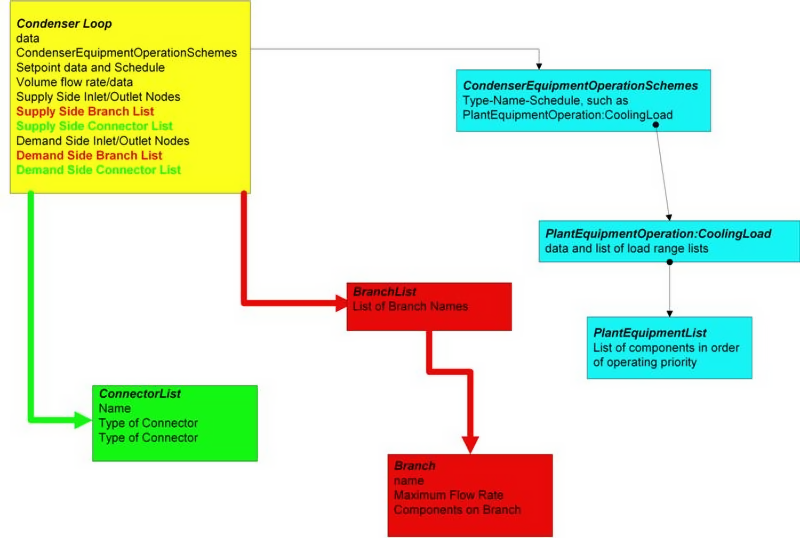
\includegraphics[width=0.9\textwidth, height=0.9\textheight, keepaspectratio=true]{media/image136.png}
\caption{Condenser Loop Input Syntax Map \protect \label{fig:condenser-loop-input-syntax-map}}
\end{figure}

\subsubsection{Inputs}\label{inputs-1-032}

\paragraph{Field: Name}\label{field-name-1-031}

This alpha field is used as an identifying field for the condenser loop.

\paragraph{Field: Fluid Type}\label{field-fluid-type-1-000}

This alpha field must be a keyword selected from the list of available fluids for an EnergyPlus plant loop. Either \textbf{Water} or \textbf{UserDefinedFluidType} may be used. If the UserDefinedFluidType keyword is used, the following input field i.e.~User Defined Fluid Type must have a value (namely the name of a \hyperref[fluidpropertiesglycolconcentration]{FluidProperties:GlycolConcentration} object).

\paragraph{Field: User Defined Fluid Type}\label{field-user-defined-fluid-type-1}

This alpha field must be specified when the previous field is set to \textbf{UserDefinedFluidType} otherwise it could be left blank. \textbf{Water}, \textbf{EthyleneGlycol}, and \textbf{PropyleneGlycol} are all ``built-in'' fluids for EnergyPlus (that is, all of the appropriate properties are contained within the program). If the fluid specified here is a mixture of water and ethylene or propylene glycol, then only \hyperref[fluidpropertiesglycolconcentration]{FluidProperties:GlycolConcentration} objects need to be specified and the name of the appropriate one is used here. For another water/glycol mixture, a complete set of fluid property data (\hyperref[fluidpropertiesname]{FluidProperties:Name} and FluidProperties:Temperature objects plus multiple \hyperref[fluidpropertiesconcentration]{FluidProperties:Concentration} objects for specific heat, density, etc.) must be specified (Ref dataset: GlycolPropertiesRefData.idf).

\paragraph{Field: Condenser Equipment Operation Scheme Name}\label{field-condenser-equipment-operation-scheme-name}

This alpha field is used as an identifying field for the condenser operation scheme. This field ties to the Condenser Operation Schemes input structure, which must also be defined.

\paragraph{Field: Condenser Loop Temperature Setpoint Node Name}\label{field-condenser-loop-temperature-setpoint-node-name}

This alpha field is used to identify the node which the Loop Manager will access the temperature setpoint that it will try to maintain. This is typically the Condenser Loop Supply Side Outlet Node so that it will not interfere with component temperature setpoints. An associated temperature setpoint manager will need to be defined.

\paragraph{Field: Maximum Loop Temperature}\label{field-maximum-loop-temperature-1}

This numeric field contains the maximum allowable temperature in Celsius for this loop.

\paragraph{Field: Minimum Loop Temperature}\label{field-minimum-loop-temperature-1}

This numeric field contains the minimum allowable temperature in Celsius for this loop. This minimum loop temperature is used by the cooling towers to make sure that the minimum is not violated to keep the equipment safe. The minimum is also used to trigger the minimum temperature warning and will notify the user if it gets too low.

\paragraph{Field: Maximum Loop Flow Rate}\label{field-maximum-loop-flow-rate-1}

This numeric field contains the maximum loop flow rate in cubic meters per second. This field is autosizable.

\paragraph{Field: Minimum Loop Flow Rate}\label{field-minimum-loop-flow-rate-1}

This numeric field contains the minimum loop flow rate in cubic meters per second.

\paragraph{Field: Condenser Loop Volume}\label{field-condenser-loop-volume}

Volume of the condenser loop in m\(^{3}\). This numeric field contains the loop volume for the entire loop, i.e., both the demand side and the supply side. This is used for the loop capacitance calculation. Loop volume (m\(^{3}\)) could be calculated from pipe size data but this is not usually known. If zero volume is specified the loop has no fluid heat capacity. If a very large capacitance is specified unrealistic time delay may result and there may be poor response to changes in loop setpoint temperature. The \textbf{autocalculate} option sets the loop volume to the product of the Maximum Loop Flow Rate and the user input for Loop Circulation Time which defaults to 2 minutes (see below). This calculation is described in the Engineering Reference manual.

\paragraph{Field: Condenser Side Inlet Node Name}\label{field-condenser-side-inlet-node-name}

This required alpha field contains the identifying name given to the Condenser Side Inlet Node. This node is the inlet to the supply side of the loop.

\paragraph{Field: Condenser Side Outlet Node Name}\label{field-condenser-side-outlet-node-name}

This required alpha field contains the identifying name given to the Condenser Side Outlet Node. This node is the outlet of the supply side of the loop.

\paragraph{Field: Condenser Side Branch List Name}\label{field-condenser-side-branch-list-name}

This required alpha field contains the identifying name given to the Condenser Side Branch List. The list referenced here should list all the branches on the supply side of the loop.

\paragraph{Field: Condenser Side Connector List Name}\label{field-condenser-side-connector-list-name}

This required alpha field contains the identifying name given to the Condenser Side Connector List.~ The list referenced here should list the splitter and mixer on the supply side of the loop.

\paragraph{Field: Demand Side Inlet Node Name}\label{field-demand-side-inlet-node-name-1}

This required alpha field contains the identifying name given to the Demand Side Inlet Node.~ This node is the inlet to the demand side of the loop.

\paragraph{Field: Demand Side Outlet Nodes Name}\label{field-demand-side-outlet-nodes-name}

This required alpha field contains the identifying name given to the Demand Side Outlet Node. This node is the outlet of the demand side of the loop.

\paragraph{Field: Condenser Demand Side Branch List Name}\label{field-condenser-demand-side-branch-list-name}

This required alpha field contains the identifying name given to the Demand Side Branch List.~ The list referenced here should list all the branches on the demand side of the loop.

\paragraph{Field: Condenser Demand Side Connector List Name}\label{field-condenser-demand-side-connector-list-name}

This required alpha field contains the identifying name given to the Demand Side Connector List. The list referenced here should list the splitter and mixer on the demand side of the loop.

\paragraph{Field: Load Distribution Scheme}\label{field-load-distribution-scheme-1-000}

This alpha field contains the Load Distribution Scheme Keyword. The Load Distribution Scheme selects the algorithm used to sequence equipment operation in order to meet the plant loop demand. Currently, five schemes are functional. \textbf{Optimal} operates each piece of equipment at its optimal part load ratio and will operate the last component between its minimum and maximum part load ratio in order to meet the loop demand. \textbf{SequentialLoad} loads each piece of equipment sequentially in the order specified in the \hyperref[plantequipmentlist]{PlantEquipmentList} to its maximum part load ratio and will operate the last required piece of equipment between its minimum and maximum part load ratio in order to meet the loop demand. \textbf{UniformLoad} evenly distributes the loop demand among all available components on the equipment list for a given load range. \textbf{SequentialUniformPLR} loads all equipment on the \hyperref[plantequipmentlist]{PlantEquipmentList} to a uniform part load ratio (PLR). Components are loaded sequentially based on the order specified in the \hyperref[plantequipmentlist]{PlantEquipmentList} until each component is fully loaded, at which point the next subsequent component is added and the load is distributed uniformly based on PLR between the components. \textbf{UniformPLR} will load all equipment on the \hyperref[plantequipmentlist]{PlantEquipmentList} to a uniform part load ratio (PLR). No equipment will be loaded below its minimum PLR. If the total load is less than the sum of all equipment on the \hyperref[plantequipmentlist]{PlantEquipmentList} operating at their respective minimum PLRs, then the last item in the equipment list is dropped and the load is distributed based on a uniform PLR for the remaining plant equipment.

Note: For all schemes, if the load for any individual component is less than the component load at the minimum PLR, the individual component model will false load or reduce duty cycle while operating at the minimum part load ratio until the load is met.

\paragraph{Field: Pressure Simulation Type}\label{field-pressure-simulation-type-1}

This field lets user to choose if this plant loop will be involved in a pressure drop calculation.~ This requires that at least one branch on the loop have pressure drop data.~ If not, an error will be thrown due to the input mismatch.~ Currently there are two pressure drop simulation types: ``PumpPowerCorrection'' and ``LoopFlowCorrection''.~ In both of these methods, branch pressure drop data is used to calculate a dynamic loop pressure drop and is used to update pumping power accordingly.~ The flow correction method allows the user to enter information regarding the pressure curve of a constant speed pump so that the simulation can dynamically resolve the pressure vs.~flow relationship in the plant loop.~ This is limited to constant speed pumps, as the variable speed pumps are expected to resolve as if it were controlled by a variable drive, so that they can inherently meet any pressure and flow demand required by the loop.~ This is also limited to ``loop pumps'', where there is a single pump on the plant loop.~ Common pipe simulations and ``branch pump'' simulations are not compatible with this level of pressure simulation.~ See the documentation for the \hyperref[pumpconstantspeed]{Pump:ConstantSpeed} in order to determine required inputs for this pressure simulation method to be performed.~ In the pressure drop system, parallel flow rates are not resolved (to match the pressure drop for the parallel system).~ Enhancements to this calculation are planned which will allow parallel branch flow resolution.~ See the Engineering Reference document for more information on how this works.

\paragraph{Field: Loop Circulation Time}\label{condenserloop-field-loop-circulation-time}

This field specifies the time it takes the fluid to circulate through the entire loop. It is only used when Condenser Loop Volume is set to autocalculate. The default is 2 minutes.

An example of this statement used in an IDF is:

\begin{lstlisting}

  CondenserLoop,
      Condenser Water Loop,    !- Name
      Water,                   !- Fluid Type
      ,                        !- User Defined Fluid Type
      Tower Loop Operation,    !- Condenser Equipment Operation Scheme Name
      Condenser Supply Outlet Node,  !- Condenser Loop Temperature Setpoint Node Name
      80,                      !- Maximum Loop Temperature {C}
      10,                      !- Minimum Loop Temperature {C}
      autosize,                !- Maximum Loop Flow Rate {m3/s}
      0.0,                     !- Minimum Loop Flow Rate {m3/s}
      autocalculate,           !- Condenser Loop Volume {m3}
      Condenser Supply Inlet Node,  !- Condenser Side Inlet Node Name
      Condenser Supply Outlet Node,  !- Condenser Side Outlet Node Name
      Condenser Supply Side Branches,  !- Condenser Side Branch List Name
      Condenser Supply Side Connectors,  !- Condenser Side Connector List Name
      Condenser Demand Inlet Node,  !- Demand Side Inlet Node Name
      Condenser Demand Outlet Node,  !- Demand Side Outlet Node Name
      Condenser Demand Side Branches,  !- Condenser Demand Side Branch List Name
      Condenser Demand Side Connectors,  !- Condenser Demand Side Connector List Name
      SequentialLoad;              !- Load Distribution Scheme

    SetpointManager:FollowOutdoorAirTemperature,
      MyCondenserControl,      !- Name
      Temperature,             !- Control Variable
      OutdoorAirWetBulb,       !- Reference Temperature Type
      0,                       !- Offset Temperature Difference {deltaC}
      80,                      !- Maximum Setpoint Temperature {C}
      10,                      !- Minimum Setpoint Temperature {C}
      Condenser Supply Outlet Node;  !- Setpoint Node or NodeList Name

    CondenserLoop,
      Chilled Water Condenser Loop,  !- Name
      UserDefinedFluidType,    !- Fluid Type
      PropyleneGlycol15Percent,!- User Defined Fluid Type
      Tower Loop Operation,    !- Condenser Equipment Operation Scheme Name
      Condenser Supply Outlet Node,  !- Condenser Loop Temperature Setpoint Node Name
      80,                      !- Maximum Loop Temperature {C}
      10,                      !- Minimum Loop Temperature {C}
      0.00330000,              !- Maximum Loop Flow Rate {m3/s}
      0,                       !- Minimum Loop Flow Rate {m3/s}
      autocalculate,           !- Condenser Loop Volume {m3}
      Condenser Supply Inlet Node,  !- Condenser Side Inlet Node Name
      Condenser Supply Outlet Node,  !- Condenser Side Outlet Node Name
      Condenser Supply Side Branches,  !- Condenser Side Branch List Name
      Condenser Supply Side Connectors,  !- Condenser Side Connector List Name
      Condenser Demand Inlet Node,  !- Demand Side Inlet Node Name
      Condenser Demand Outlet Node,  !- Demand Side Outlet Node Name
      Condenser Demand Side Branches,  !- Condenser Demand Side Branch List Name
      Condenser Demand Side Connectors,  !- Condenser Demand Side Connector List Name
      SequentialLoad;              !- Load Distribution Scheme
\end{lstlisting}

\subsubsection{Outputs}\label{outputs-1-018}

\begin{itemize}
\item
  HVAC,Average,Plant Supply Side Cooling Demand Rate {[}W{]}
\item
  HVAC,Average,Plant Supply Side Heating Demand Rate {[}W{]}
\item
  HVAC,Average,Plant Supply Side Inlet Mass Flow Rate {[}kg/s{]}
\item
  HVAC,Average,Plant Supply Side Inlet Temperature {[}C{]}
\item
  HVAC,Average,Plant Supply Side Outlet Temperature {[}C{]}
\item
  HVAC,Average,Cond Loop Demand Not Distributed {[}W{]}
\item
  HVAC,Average,Plant Supply Side Unmet Demand Rate {[}W{]}
\item
  HVAC,Average,Plant Demand Side Loop Pressure Difference {[}Pa{]}
\item
  HVAC,Average,Plant Supply Side Loop Pressure Difference {[}Pa{]}
\item
  HVAC,Average,Plant Loop Pressure Difference {[}Pa{]}
\end{itemize}

\paragraph{Plant Supply Side Cooling Demand Rate {[}W{]}}\label{plant-supply-side-cooling-demand-rate-w-1}

This is the value of the net demand required to meet the cooling setpoint of the loop.~ If the loop setpoint is met for the current HVAC timestep, Plant Supply Side Cooling Demand Rate will equal sum of the total cooling demand from the demand side components on the loop (typically condenser coils of chillers, etc.).~ It will also equal the cooling output of all condensing equipment such as cooling towers on the loop less any pump heat added to the fluid.~ For example, for a condenser loop with one tower and one pump serving one chiller, Plant Supply Side Cooling Demand Rate will equal the tower water-side heat transfer less the pump heat to fluid, and it will also equal the chiller condenser heat transfer rate.

If the condenser loop setpoint is not met, Plant Supply Side Cooling Demand Rate will equal the sum of the total cooling demand from the demand side components on the loop plus the additional cooling required to bring the loop flow to setpoint.~ If the loop remains off setpoint for successive timesteps, the demand required to return to setpoint will repeat in each timestep until the loop reaches setpoint.~ For this reason, Plant Supply Side Cooling Demand Rate should not be summed over time, because it will overstate the demand whenever the loop is off setpoint.

\paragraph{Plant Supply Side Heating Demand Rate {[}W{]}}\label{plant-supply-side-heating-demand-rate-w-1}

This is the value of the net demand required to meet the heating setpoint of the loop.~ If the loop setpoint is met for the current HVAC timestep, Plant Supply Side Heating Demand Rate will equal sum of the total heating demand from the demand side components on the loop.~ It will also equal the heating output of all heating equipment on the supply side of the loop plus any pump heat added to the fluid.~ For example, for a condenser loop with one ground loop heat exchanger and one pump serving one water-to-water heat pump, Plant Supply Side Heating Demand Rate will equal the ground loop heat transfer plus the pump heat to fluid, and it will also equal the heat pump condenser side heat transfer rate.

If the condenser loop setpoint is not met, Plant Supply Side Heating Demand Rate will equal the sum of the total heating demand from the demand side components on the loop plus the additional heating required to bring the loop flow to setpoint.~ If the loop remains off setpoint for successive timesteps, the demand required to return to setpoint will repeat in each timestep until the loop reaches setpoint.~ For this reason, Plant Supply Side Heating Demand Rate should not be summed over time, because it will overstate the demand whenever the loop is off setpoint.

\paragraph{Plant Supply Side Inlet Mass Flow Rate {[}kg/s{]}}\label{plant-supply-side-inlet-mass-flow-rate-kgs-1}

This is the value of the mass flow rate at the Inlet to Condenser Loop on the supply side. There is not an associated Condenser Loop outlet node flow rate since continuity must be maintained in the loop and the outlet must be the same.

\paragraph{Plant Supply Side Inlet Temperature {[}C{]}}\label{plant-supply-side-inlet-temperature-c-1}

This is the value of the temperature at the Inlet to the condenser loop on the supply side.

\paragraph{Cond Loop OutletNode Temperature {[}C{]}}\label{cond-loop-outletnode-temperature-c}

This is the value of the temperature at the outlet to the condenser loop on the supply side.

\paragraph{Cond Loop Demand Not Distributed {[}W{]}}\label{cond-loop-demand-not-distributed-w}

This is the value of the demand that could not be distributed to the condenser equipment because of some constraint in the operation scheme.~ This is a record of the loop operation scheme supervisory controls after attempting to distribute the load.~ For example it would be~ non-zero in situations where the load is larger than the upper limit of capacities set for the condenser equipment controls.~ This output is for \emph{before} the equipment has actually been simulated whereas the separate output Plant Supply Side Unmet Demand Rate is for \emph{after} the equipment has simulated.

\paragraph{Plant Supply Side Unmet Demand Rate {[}W{]}}\label{plant-supply-side-unmet-demand-rate-w-1}

This is the value of the demand NOT provided by the condenser equipment to meet the heating or cooling setpoint of the loop. The value is positive when the condenser equipment cannot meet the setpoint, and the value is negative when the condenser equipment provides more than enough heating or cooling to meet the setpoint. A negative value can happen when the amount of demand is smaller than the minimum capacity of the equipment using the minimum part load ratio.

\paragraph{Plant Demand Side Loop Pressure Difference {[}Pa{]}}\label{plant-demand-side-loop-pressure-difference-pa-1}

This field is the demand side pressure drop of a condenser loop.~ This output is only recognized if a valid pressure simulation is being performed.~ To do this, the user must specify a pressure simulation type as an input in the CondenserLoop object, and input at least one pressure drop curve on a branch of the plant/condenser loop.~ This particular output is only relevant if the user puts that curve on the demand side of the loop.

\paragraph{Plant Supply Side Loop Pressure Difference {[}Pa{]}}\label{plant-supply-side-loop-pressure-difference-pa-1}

This field is the supply side pressure drop of a condenser loop.~ This output is only recognized if a valid pressure simulation is being performed.~ To do this, the user must specify a pressure simulation type as an input in the CondenserLoop object, and input at least one pressure drop curve on a branch of the plant/condenser loop.~ This particular output is only relevant if the user puts that curve on the supply side of the loop.

\paragraph{~Plant Loop Pressure Difference {[}Pa{]}}\label{plant-loop-pressure-difference-pa-1}

This field is the total pressure drop of a condenser loop.~ This output is only recognized if a valid pressure simulation is being performed.~ To do this, the user must specify a pressure simulation type as an input in the CondenserLoop object, and input at least one pressure drop curve on a branch of the plant/condenser loop.~ This particular output is relevant regardless of the location of pressure drop curves: demand side, supply side, or both.
